% \documentclass[rnd]{mas_proposal}
\documentclass[thesis]{mas_proposal}

\usepackage[utf8]{inputenc}
\usepackage{amsmath}
\usepackage{amsfonts}
\usepackage{amssymb}
\usepackage{graphicx}
\usepackage{pdflscape}
\usepackage{svg}

\title{Federated Learning for Object Detection Using 3D Depth Images}
\author{Kevin Patel}
\supervisors{Prof. Dr.-Ing. Sebastian Houben\\Prof. Dr. Robert Lange\\Dr. Markus Hammes\\Dr. Nikolaus Mayer}
\date{September 2024}

\thirdpartylogo{images/Logo_SICK_AG_2009.png}

\begin{document}

\maketitle

\pagestyle{plain}

\section{Introduction}

\subsection{Topic of This Thesis}
\begin{itemize}
      % *************************
      \item Provide reasonably detailed description of what you intent to do in your R\&D project.
      \item You may also discuss the challenges that you have to address.
      \item Reflect on the profile of the reader and PLEAAAASE, tell a story here and refrain from bombarding the readers with details which they may not be able to appreciate.
      % **************************

      %     \item Imagine driving on a winding mountain road at night, with fog and rain obscuring your view, your vehicle's self-driving system struggles to detect objects ahead due to the challenging weather conditions. Suddenly, a deer jumps out in front of your car, causing the system to issue an alert and apply the brakes in time to avoid a collision.
      \item TODO: Put a story or a very basic scenario here to make the reader understand the problem.
      \item Keep it in industrial context
      \item Start with privacy issue with the centralized training especially in the consumer AI context
      \item Issue with scaling DL models
      \item Then how FL solves that problem, put a FL workflow diagram
      \item FL settings, what is our focus in that
      \item Industrial context
      \item Applicable to broader fields, medical, finance, surveillance
      \item Laws enforcing FL, put those papers
            \begin{itemize}
                  \item \cite{voigt2017eu}
            \end{itemize}

            % TODO: add as many as good images possible in the doc
            % \begin{figure}[h]
            %       \centering
            %       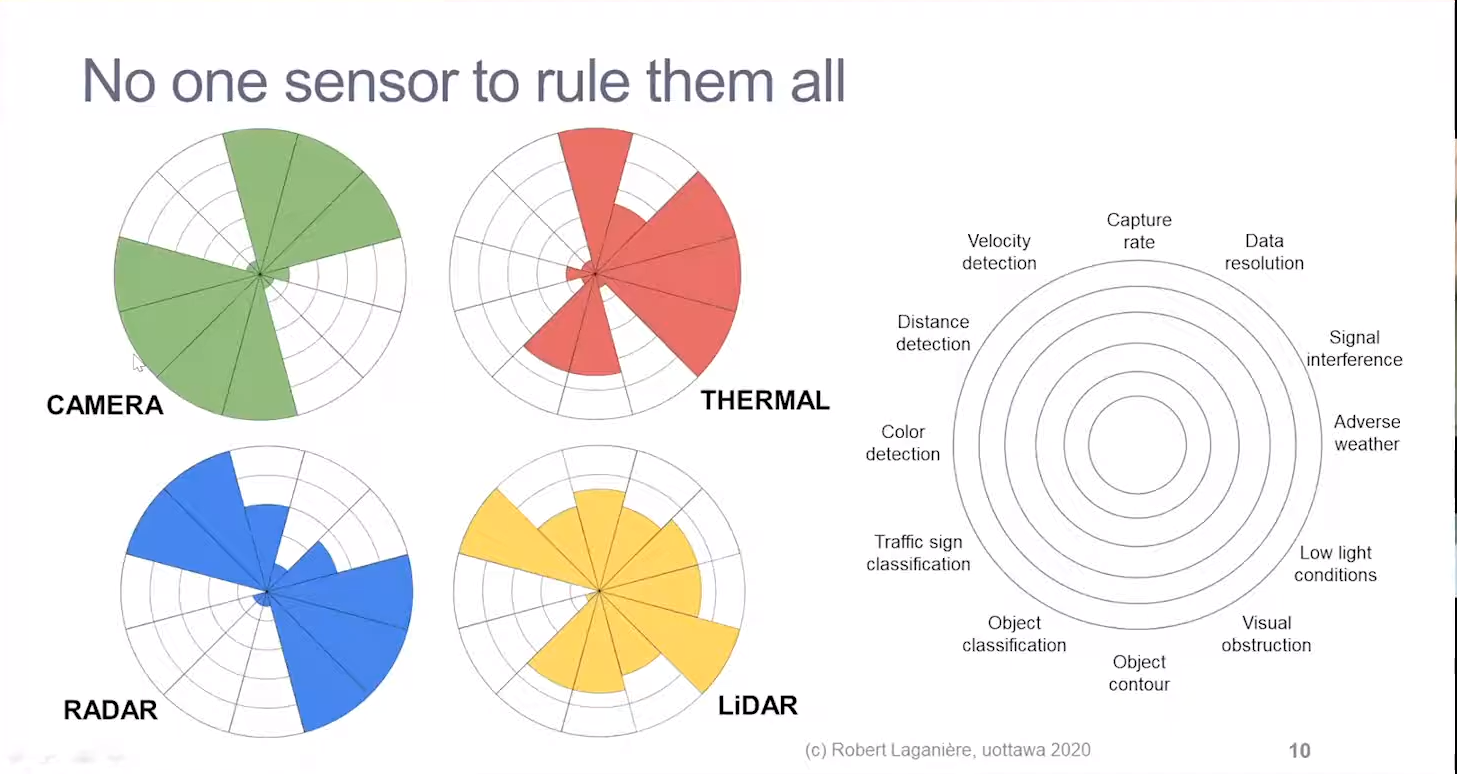
\includegraphics[width=0.7\textwidth]{images/sensors_intro_1.png}
            %       \caption{Sensors modality characteristics \cite{Sensor_modality_characteristics_1}}
            %       \label{fig:sensors_intro_1}
            % \end{figure}

\end{itemize}

\subsection{Relevance of This R\&D Project}
\begin{itemize}

      % *************************    
      \item Who will benefit from the results of this R\&D project?
      \item What are the benefits? Quantify the benefits with concrete numbers.
            % *************************
\end{itemize}

\section{Related Work}

\subsection{Survey of Related Work}
\begin{itemize}

      % - Overall talk about:
      %     - 

      % - TODO:
      %     - First, start with writing all the information about the related work
      %     - Later, we can organize it into proper sequence
      %     - Stop when you find at least 10 related papers.

      % ***********************
      \item What have other people done to solve the problem?
      \item You should reference and briefly discuss at least the ``top twelve'' related works
      \item Rising research trend for FL, put that fig with papers over years
      \item But mostly theoretical aspect on benefits of FL and its comparison with some toy datasets 
      \item FL+CV, only classification is covered in most of the papers, show that paper published graphs
      \item A very few FL+OD papers, that to even in practical and application oriented are close to none
      
            % ***********************
\end{itemize}

\subsection{Limitation and Deficits in the State of the Art}
\begin{itemize}


      % ***********************
      \item List the deficits that you have discovered in the related work and explain them such that a person who is not deep into the technical details can still understand them.
            For each deficit, provide at least two references
      \item You should reference and briefly discuss at least the ``top twelve'' related works
      \item None in the 3D depth image domain or intensity images
      \item Here, input data itself prioritize privacy especially when it comes to person recognition
            % ***********************
\end{itemize}

\section{Problem Statement}
\begin{itemize}

      % ########################################################
      % ###################################################
      % BOOKMARK: 
      % 1. Start writing problem statement - Pending
      % 2. Rephrase the related work paragraphs - Pending
      % 3. Write the project plan - DONE
      % 4. Generate Gantt chart - Pending
      % ########################################################
      % ########################################################

      \item Which of the deficits are you going to solve?
      \item What is your intended approach?
      \item How will you compare you approach with existing approaches?
      \item FL+OD working pipeline, on a real world dataset
      \item A non-RGB based dataset
      \item Implementation on edge-devices
      \item Compare FL frameworks and choose 1 or 2
      \item Check FL aggregation methods
      \item Analyze compute resource constrained OD models
      
      % ////////////////////////////
      \item As seen in the Figure (TODO: add a figure with computer vision task papers), most of the literature work is done in federated learning (FL) for computer vision is for classification. FL with object detection is not yet well explored with the new edge hardware and the state-of-the-art models.

            % \item The comparative analysis of the results will include an assessment of the strengths and weaknesses of each approach with respect to existing state-of-the-art methods.

\end{itemize}

\section{Project Plan}

\subsection{Work Packages}
% \emph{Planning is the replacement of randomness by error.} (Einstein). Very much like you would never start a longer journey without a detailed travel plan, you should not start a project without a carefully though out work plan. A work package is a logical decomposition of a larger piece of work into smaller parts following a ``divide and conquer" strategy. It is very specific to the problem that you are going to address. Refrain from a rather generic decomposition. If your work plan looks similar to those of your school mates, which may address completely different problems then you have not thought carefully enough about how you approach the problem. It is ok to have two generic work packages \emph{Literature Study} and \emph{Project Report}. Discuss your work packages in the ASW seminar.

% The bare minimum will include the following packages:
\begin{enumerate}

      \item[WP1] Literature Study
            \begin{itemize}
                  \item[WP1.1] Conduct a comprehensive literature review on state-of-the-art FL-based object detection methods
                  \item[WP1.2] Analyze existing centralized and FL-based object detection frameworks, focusing on their architectures and performance metrics
                  \item[WP1.3] Identify key models and techniques to replicate and compare, and document best practices for FL in the context of object detection on 3D depth images
            \end{itemize}

      \item[WP2] Data Collection and Preparation
            \begin{itemize}
                  \item[WP2.1] Generate a custom dataset consisting of 3D depth images suitable for training and testing object detection models
                  \item[WP2.2] Preprocess the dataset, including data cleaning, augmentation, and handling any data imbalance issues
                  \item[WP2.3] Develop tools for managing and preparing the dataset for Federated Learning experiments (e.g., partitioning the dataset across simulated nodes)
            \end{itemize}

      \item[WP3] Model Development and Initial Testing
            \begin{itemize}
                  \item[WP3.1] Replicate and test existing models from the literature to establish a baseline performance on the custom dataset
                  \item[WP3.2] Implement the FL-based object detection pipeline, starting with a centralized approach for comparison
                  \item[WP3.3] Test and evaluate initial models to ensure functionality and establish initial performance benchmarks
            \end{itemize}

      \item[WP4] Comparative Analysis and Performance Evaluation
            \begin{itemize}
                  \item[WP4.1] Perform a comparative analysis between centralized and FL-based object detection methods, focusing on performance metrics such as accuracy, inference time, and system profile
                  \item[WP4.2] Evaluate models on the custom dataset and analyze the strengths and weaknesses of each approach
                  \item[WP4.3] Optimize model performance by tuning hyperparameters, modifying architecture, or adjusting the dataset for improved FL-based results
            \end{itemize}

      \item[WP5] Implementation on Edge Devices
            \begin{itemize}
                  \item[WP5.1] Implement the FL-based object detection model on edge devices, ensuring it runs efficiently under resource constraints (e.g., limited computation, bandwidth)
                  \item[WP5.2] Test and evaluate the performance of the model on edge devices, measuring factors such as accuracy, inference time, and system profile
                  \item[WP5.3] Integrate any necessary optimizations for FL-based object detection specifically tailored to edge deployment scenarios
            \end{itemize}

      \item[WP6] Advanced Development and Optional Extensions
            \begin{itemize}
                  \item[WP6.1] Develop a containerized workflow to facilitate easy deployment of the FL-based object detection pipeline across different environments
                  \item[WP6.2] If time permits, extend the project by integrating object tracking with FL-based object detection or adding uncertainty estimation capabilities to the models
            \end{itemize}

      \item[WP7] Project Report and Finalization
            \begin{itemize}
                  \item[WP7.1] Write a comprehensive project report detailing the research objectives, methodology, results, and findings
                  \item[WP7.2] Present a critical analysis of the performance comparison between centralized and FL-based approaches, highlighting contributions, limitations, and future research directions
                  \item[WP7.3] Prepare the final thesis draft, ensuring clarity and coherence in presenting the experimental outcomes and their implications for FL-based object detection
            \end{itemize}

\end{enumerate}

\subsection{Milestones}
% Milestones mark the completion of a certain activity or at least a major achievement in an activity. Milestones are also decision points, where you reflect on what you have achieved and what options you have for continuing your work in case you have not achieved what was planned. Above all, milestones have to be measurable. As above, if your milestones are the same as those of your school mates, then you may not have thought carefully enough about how your project shall progress.

\begin{enumerate}
      \item[M1] Comprehensive literature review on state-of-the-art FL-based object detection methods completed, with key models and techniques identified for replication
      \item[M2] Replication of existing models from relevant literature completed
      \item[M3] Custom 3D depth image dataset generated and preprocessed (e.g., cleaning, augmentation)
      \item[M4] Comparative analysis of at least two object detection methods on the custom dataset completed, with detailed performance metrics recorded
      \item[M5] Development of a working pipeline for FL-based object detection (simulated) on 3D depth images completed
      \item[M6] Implementation of FL-based object detection on edge devices completed
      \item[M7] Comparative analysis of centralized vs. FL-based object detection completed, with performance results and key findings documented
      \item[M8] Final model development and testing completed, including optimization and an in-depth evaluation of strengths and weaknesses
      \item[M9] Extension of the project with the development of a containerized workflow for easy deployment completed
      \item[M10] Final project report completed, covering methodology, experimental setup, results, and thorough analysis.
\end{enumerate}

\subsection{Project Schedule}
% Include a Gantt chart here. It doesn't have to be detailed, but it should include the milestones you mentioned above.
% Make sure to include the writing of your report throughout the whole project, not just at the end.

\begin{figure}[h]
      % \centering
      \hspace{-4em}
      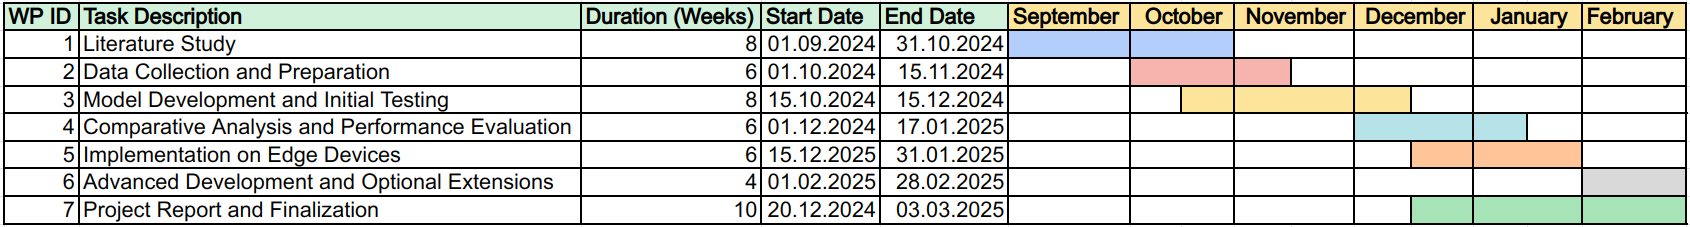
\includegraphics[scale=0.3]{images/project_plan/Gantt_chart.png}
      \caption{Gantt chart of the project schedule}
      \label{fig:myfigure}
\end{figure}

\newpage
\subsection{Deliverables}
\subsubsection*{Minimum Viable}
\begin{itemize}
      % \item Project results required to get a satisfying or sufficient grade.
      \item Conduct a comprehensive literature review on state-of-the-art Federated Learning (FL)-based object detection methods
      \item Develop and test existing models to reproduce results from relevant literature
      \item Generation of a custom dataset consisting of 3D depth images
      \item Perform a comparative analysis of at least two methods on a custom dataset
      \item Produce a detailed project report that summarizes the work done and the obtained results

\end{itemize}

\subsubsection*{Expected}
\begin{itemize}
      % \item Project results required to get a good grade.
      %     \item Compare with more advance methods with baseline methods on different datasets
      %     \item Compare with more advance methods with baseline methods
      \item Fulfill all minimum viable deliverables
      \item Perform a comparison of centralized versus FL-based object detection, focusing on performance analysis
      \item Complete the final development and testing of the model, and a detailed analysis of the strengths and weaknesses of each approach
      \item Develop a working pipeline for FL-based object detection on 3D depth images (simulated)
      \item Produce a more extensive project report detailing the methodology, experimental setup, results, and in-depth analysis

\end{itemize}

\subsubsection*{Desired}
\begin{itemize}
      % \item Project results required to get an excellent grade.
      \item Fulfill all expected deliverables
      \item Implement FL-based object detection on edge devices
      \item Develop a containerized workflow for easy deployment
      \item Additional objectives (if time permits):
      \begin{itemize}
            \item Integrate object tracking with FL-based object detection
            \item Implement FL-based object detection with uncertainty estimation
      \end{itemize}

\end{itemize}

% Please note that the final grade will not only depend on the results obtained in your work, but also on how you present the results.

\nocite{*}

\bibliographystyle{unsrt} % Use the plainnat bibliography style
\bibliography{bibliography.bib} % Use the bibliography.bib file as the source of references

\end{document}